\documentclass[sigconf]{acmart}
\settopmatter{printacmref=true} % Removes citation information below abstract
%\renewcommand\footnotetextcopyrightpermission[1]{} % removes footnote with conference information in first column
\usepackage{balance} 
\usepackage{booktabs} % For formal tables
\usepackage[vlined,linesnumbered,ruled,noend]{algorithm2e}     % algorithms
\usepackage[show]{chato-notes}
\usepackage{natbib}
\usepackage{tikz}
\usetikzlibrary{automata,arrows,positioning,calc}
\usepackage{lipsum}% http://ctan.org/pkg/lipsum
\usepackage{multicol}% http://ctan.org/pkg/multicols
\usepackage{float}
\usepackage{wrapfig}

% notations
\renewcommand{\vec}[1]{\mathbf{#1}} % vector
\newcommand{\matr}[1]{\mathbf{#1}} % matrix
\newcommand{\transpose}[1]{\mathbf{#1}^\intercal} % transpose

% Dot product notation
\makeatletter
\newcommand*\bigcdot{\mathpalette\bigcdot@{.5}}
\newcommand*\bigcdot@[2]{\mathbin{\vcenter{\hbox{\scalebox{#2}{$\m@th#1\bullet$}}}}}
\makeatother

% strategies
\newcommand{\naive}{{\textsc{Naive Strategy}}}
\newcommand{\relocation}{{\textsc{Relocation Strategy}}}
\newcommand{\flexible}{{\textsc{Flexible Schedule Strategy}}}
\newcommand{\relocationflexible}{{\textsc{Relocation with Flexible Schedule Strategy}}}

% actions
\newcommand{\getpassenger}{{\sc Get Passenger}}
\newcommand{\gohome}{{\sc Go Home}}
\newcommand{\relocate}{{\sc Relocate}}

%symbols
\newcommand{\parents}{\ensuremath{\pi}}
\newcommand{\children}{\ensuremath{\kappa}}
\newcommand{\transition}{\ensuremath{\mathbf{P}}}
\newcommand{\steadystate}{\ensuremath{\mathbf{p}}}
\newcommand{\initial}{\ensuremath{\mathbf{x}}}
\newcommand{\final}{\ensuremath{\mathbf{z}}}
\newcommand{\uncertainty}{\ensuremath{F}}
\newcommand{\objective}{\ensuremath{\mathbf{F}}}
\newcommand{\variance}{\ensuremath{\mathbf{var}}}
\newcommand{\rvFinal}{\ensuremath{\mathbf{Z}}}
\newcommand{\actualtransitions}{\ensuremath{\mathbf{T}}}
\newcommand{\prob}{\ensuremath{\mathbf{Pr}}}

\DeclareMathOperator*{\argmin}{arg\,min}
\DeclareMathOperator*{\argmax}{arg\,max}

\newcommand{\etal}{\emph{et al.}}

%formating
\newcommand{\spara}[1]{\smallskip\noindent{\bf{#1}}}
\newcommand{\mpara}[1]{\medskip\noindent{\bf{#1}}}
\newcommand{\bpara}[1]{\bigskip\noindent{\bf{#1}}}


\begin{document}
\copyrightyear{2018} 
\acmYear{2018} 
\setcopyright{acmcopyright}
\acmConference[WSDM 2018]{WSDM 2018: The Eleventh ACM International Conference on Web Search and Data Mining }{February 5--9, 2018}{Marina Del Rey, CA, USA}
\acmBooktitle{WSDM 2018: WSDM 2018: The Eleventh ACM International Conference on Web Search and Data Mining , February 5--9, 2018, Marina Del Rey, CA, USA}
\acmPrice{15.00}
\acmDOI{10.1145/3159652.3159721}
\acmISBN{978-1-4503-5581-0/18/02}


\title{Putting Data in the Driver's Seat:\\
Optimizing Earnings for On-Demand Ride-Hailing}
% \titlenote{Produces the permission block, and copyright information}
% \subtitle{Extended Abstract}


\author{Harshal A. Chaudhari}
\affiliation{%
 \institution{Boston University}
}
\email{harshal@cs.bu.edu}

\author{John W. Byers}
\affiliation{%
 \institution{Boston University}
}
\email{byers@cs.bu.edu}

\author{Evimaria Terzi}
\affiliation{%
 \institution{Boston University}
}
\email{evimaria@cs.bu.edu}

% The default list of authors is too long for headers}
% \renewcommand{\shortauthors}{F. Lastname et al.}

%
% The code below should be generated by the tool at
% http://dl.acm.org/ccs.cfm
% Please copy and paste the code instead of the example below. 
%
% \begin{CCSXML}
% <ccs2012>
%  <concept>
%   <concept_id>10010520.10010553.10010562</concept_id>
%   <concept_desc>Computer systems organization~Embedded systems</concept_desc>
%   <concept_significance>500</concept_significance>
%  </concept>
%  <concept>
%   <concept_id>10010520.10010575.10010755</concept_id>
%   <concept_desc>Computer systems organization~Redundancy</concept_desc>
%   <concept_significance>300</concept_significance>
%  </concept>
%  <concept>
%   <concept_id>10010520.10010553.10010554</concept_id>
%   <concept_desc>Computer systems organization~Robotics</concept_desc>
%   <concept_significance>100</concept_significance>
%  </concept>
%  <concept>
%   <concept_id>10003033.10003083.10003095</concept_id>
%   <concept_desc>Networks~Network reliability</concept_desc>
%   <concept_significance>100</concept_significance>
%  </concept>
% </ccs2012>  
% \end{CCSXML}
% 
% \ccsdesc[500]{Computer systems organization~Embedded systems}
% \ccsdesc[300]{Computer systems organization~Redundancy}
% \ccsdesc{Computer systems organization~Robotics}
% \ccsdesc[100]{Networks~Network reliability}

% We no longer use \terms command
%\terms{Theory}

%!TEX root = main.tex

\begin{abstract}
On-demand ridesharing platforms like Uber and Lyft play an important role in urban transportation, 
  enabling car owners to become drivers for hire with minimal overhead.
One natural optimization problem in this domain has focused on optimal route planning of a deployed
  fleet of vehicles, with objective functions geared largely towards improving the overall service 
  to passengers or minimizing total resource utilization (fuel consumption, miles driven, etc.).
But much less emphasis has been placed on optimization for individual drivers.
While some individuals drive opportunistically either as their schedule allows or on a fixed 
  schedule, strategic behavior regarding when and where to drive can substantially increase
  driver income.
To address this issue, we model the passenger seeking behavior of the 
%% drivers on Uber are NOT taxi drivers
%%
%%taxi
drivers on Uber as a controlled Markov Decision Process (MDP) over a finite horizon of time.
%
\todo[JB]{These next sentences are too vague.  Describe more specifics and why they matter.}
The parameters of this MDP are set using Uber Rider API and publicly available New York Taxi datasets. Using this model, we devise three optimal in expectation strategies for drivers and evaluate them. Furthermore, we provide a sensitivity analysis of these strategies to account for uncertainties in the MDP parameters.
Our main finding is XXX.
\end{abstract}


% \keywords{ACM proceedings}

\maketitle
%%%!TEX root = main.tex

\subsection*{Notation}
\label{sec:notation}

Vectors are denoted with lowercase bold letters (e.g., $\vec{a} = [a(i)]$) and matrices are denoted with uppercase bold letters (e.g., $\matr{A} = [a(i,j)]$). The notation $\vec{1}$ refers to the vector of ones, with size dependent on the context. The short form notation $\vec{A_i}$ refers to the $i$-th row vector of the matrix $\matr{A}$. Let $\Theta_n$ be a set of $n \times n$ right-stochastic transition matrices (non-negative matrices with rows that sum to one). A probability simplex in $\mathbb{R}^n$ is denoted by $\Delta_n = \{\vec{p} \in \mathbb{R}^n_+ : \transpose{p} \vec{1} = 1 \}$.
  [JB: this does not go here]
%!TEX root = main.tex

\section{Introduction}
\label{sec:introduction}

The proliferation of on-demand ridesharing platforms like Lyft and Uber
  has begun to fundamentally change the nature of urban transit. 
In the last two years alone, the number of daily trips using ridesharing 
  platforms like Uber and Lyft in NYC has grown five-fold, 
  to about 350,000 trips per day. 
Today, over 65,000 drivers drive in the streets of NYC as Uber or Lyft drivers.
The explosive growth of these ridesharing platforms has motivated a wide
  array of questions for academic research at the intersection of computer
  science and economics, ranging from the design of effective pricing mechanisms, 
  to equilibrium analysis, to the design of reputation management systems for 
  drivers, to algorithms for matching drivers with 
  customers, as we discuss in our related work section.
%%~\cite{banerjee2015pricing,ozkan2016dynamic}.

While these studies consider the study of ridesharing platforms holistically, 
   little work has been done on optimizing strategies for individual drivers. 
Nevertheless, the challenge of how to maximize one's individual earnings as a driver for a 
ridesharing platform like Uber or Lyft is a pressing question that millions of micro-entrepreneurs 
across the world now face.  Anecdotally, many drivers spend a great deal of time 
strategizing about where and when to drive.  However, drivers today are 
self-taught, using heuristics of their own devising or learn from one another, 
and employ relatively simple analytics dashboards such as SherpaShare.
Indeed, rumors suggest that some drivers even collude in attempts to induce spikes in surge prices that they can then exploit.
But in terms of concrete guidance, to date there are only articles in the
  popular press and on blogs that offer (often contradictory) advice to ridesharing drivers 
  how to maximize their earnings~\cite{dont,tips,sherpashareNYT}.

In this paper, we formalize the problem of devising a driver strategy to maximize expected 
 earnings and describe a series of dynamic programming algorithms to solve this problem
 under different sets of modeled actions available to the drivers. 
Our strategies take as input a detailed model of city-level data that constitutes a 
  fine-grained weekly projection of forecasted demand for rides, comprising 
  predicted spatiotemporal distributions of source-destination pairs, driver payments,
  transit times, and surge multipliers. 
The optimization framework we propose not only produces contingency plans in the form of
  highly optimized driving schedules and real-time in-course corrections to drivers, but 
  also enables us to rigorously reason about and analyze the sensitivity of our output 
  results to perturbations in the input data.  
Thus, we can justify the proposed strategies even under an uncertainty level in the
  collected data and the data model itself.
  
We then exemplify our  results with a large-scale simulation of driving for Uber in NYC. 
For this simulation, we assemble a new dataset that uses both the publicly available NYC taxi rides 
dataset~\footnote{\url{http://www.nyc.gov/html/tlc/html/about/trip_record_data.shtml}} as well as calls to the Uber API.
From the former, we obtain information about over 200,000 taxi rides that occurred between different NYC zones. 
From the latter, we obtain representative pricing and traffic-time information for those trips, were they to reoccur on Uber.
From this newly-collected dataset, we construct a mathematical model to produce input to our algorithms. 
However, we view the dataset, which we plan to release, to be of independent interest that could subsequently 
be used for a multitude of other studies.

Our experiments with our methods on this dataset demonstrate the following findings:
being strategic about the areas they focus on picking up riders and the times they work, 
can significantly increase a driver's income, sometimes by
as much as 2x, when compared to a naive optimization strategy.
Moreover, we show that a pronounced difference between the earnings obtained by the 
two strategies holds even when there is a large uncertainty in the input data. 
We argue that our results are therefore not purely an artifact of the NYC dataset we employ, 
  but also that they have high potential to generalize well.
Finally, our experiments show that naively chasing surging prices does not typically lead 
  to significant earnings gains, but it can even introduce large opportunity costs, as drivers
  waste time driving to subsiding surges. 

%!TEX root = main.tex

\section{Related Work}
\label{sec:related_work}

To the best of our knowledge, we are the first to formally address the problem of optimizing
the driver's strategy in ride-hailing platforms like Uber and Lyft. 
Apart from 
some recent popular-press articles that 
offer, often contradictory, advice to ride-hailing drivers on how to maximize earnings, mostly via chasing surge~\cite{dont,tips}, 
the only relevant existing technical work 
studies other aspects of ride-hailing. 
Next, we discuss these works as well as some work related to optimization problems
for taxi fleets.
%Also related can be considered existing work on optimization problems related to taxi fleets. We discuss existing works along these lines next.


\spara{Studies of ride-hailing platforms:}
Recent work has investigated the supply-side effects of specific incentives (e.g., surge pricing) that Uber and Lyft provide to drivers~\cite{slaves}.  For example, Chen and Sheldon~\cite{chen2016dynamic} showed a causal relationship that drivers on Uber respond to surges by driving more during high surge times,  differentiating from previous work that suggests taxi drivers primarily focus on achieving earnings goals~\cite{camerer1997labor}. 
%Other work has viewed ride-hailing platforms more holistically, at a macro level.
In another line of research,
Chen {\etal}~\cite{chen2015peeking} measured many facets of Uber in NYC, including the prevalence and extent 
  of surge pricing.
Hall and Krueger~\cite{hall2016analysis} showed that drivers were attracted to the Uber platform due to the flexibility it offers, 
and the level of compensation, but that earnings per hour do not vary much with the number of hours worked. 
Finally, Castillo {\etal}~\cite{castillo2017surge} recently showed that surge pricing is responsible for effectively 
  relocating drivers during periods of high-demand thereby preventing them from engaging in `wild goose chases' 
  to pick up distant customers, which only exacerbates the problem of low driver availability.
These studies perform an {\em a posteriori} analysis of the data,
but they do not focus on devising specific recommendations for drivers as we do.


 In another line of work, Banerjee {\etal}~\cite{banerjee2015pricing} studied  
 dynamic
pricing strategies for ride-hailing platforms (such as Lyft) using a 
queuing-theoretic economic model. 
They showed that dynamic pricing is robust to changes in system parameters, even if it does not 
  achieve higher performance than static pricing.  
More recently, Ozkan and Ward~\cite{ozkan2016dynamic} looked at strategic matching between supply (individual drivers) 
  and demand (requested rides) for Uber and Lyft.
They showed that matching based on time-varying parameters like driver and customer arrival rates,  and
willingness of customers to wait can achieve better performance than naively matching 
passengers with the closest driver. 
Although these works build interesting models for ride-hailing economies, they are
orthogonal to ours, as they take a holistic view of such economies, while we focus 
 on earnings of individual, self-interested drivers.




\spara{Optimization problems for taxi fleets:}
A considerable body of work has focused on the optimization of taxi fleets, for
example building economic network models to describe demand and supply equilibria of taxi 
services under various tariff structures, fleet size regulations, and other policy
alternatives~\cite{bailey1987simulation,yang2002demand}.  Other work seeks to 
 optimize the allocation of taxi market resources~\cite{shi2016optimization}.
Another direction focuses on route optimization by a centralized administrator (e.g., taxi dispatching services)~\cite{maciejewski2013simulation,nunes2011taxi} 
or on maximizing occupancy and minimizing travel times 
%(by minimizing passenger detours) 
in a shared-ride setting~\cite{jung2013design}.
Other work has studied the supply side of the driving market from the viewpoint of behavioral economics.
A seminal paper by Camerer {\etal}~\cite{camerer1997labor} studied cab drivers and found that  inexperienced
cab drivers (1) make labor supply decisions ``one day at a time'' instead of substituting labor and leisure across multiple days, and  (2) set a loose daily income target and quit working once they reach that target.  
These works, however, do not focus on the design of a specific gain-optimizing
strategy for drivers, as we do.

\begin{comment}

\textbf{Works on general taxi cabs:}

2. \cite{yang1998network} - first in the series of works modeling taxi utilization and movement to find that higher utilization leads to longer waiting times for customers.

3. \cite{wong2001modeling} - second paper, extends previous paper to incorporate effects of congestion and customer demand elasticity. 

4. \cite{yang2002demand} - third paper, uses the network model to describe demand and supply equilibrium of taxi services under fare structure and fleet size regulation in competitive / monopoly market.

5. \cite{bailey1987simulation} - directed at understanding the dynamic interaction between demand, service rates, and policy alternatives. Finds that customer waiting time is insensitive to changes in demand but highly sensitive to changes in taxi fleet size.

6. \cite{qin2017mining} - explore the factors affecting driver incomes with quantitative estimates using GPS traces of over 167 million trips in Shanghai.

7. \cite{rong2016rich} - MDP to increase the revenue per unit time of taxi drivers. They study the relocate action from our strategy.

\textbf{Works on taxi routing:}

8. \cite{maciejewski2013simulation} - optimizes taxi routing by generating demand and congested network simulation. Defines online and offline taxi dispatching strategies and evaluate them. `No-scheduling' strategy works well under low demand but deteriorates under heavy load.

9. \cite{nunes2011taxi} - formulates a TSP problem to find the best route for a taxi company to satisfy demand.

\textbf{Works on ride-hailing:}

10. \cite{agatz2012optimization} - outline optimization challenges in developing technology to support ride-hailing services. Survey of operations research papers in the domain.

11. \cite{santos2013dynamic} - Prove that problem of maximizing shared trips within a fixed time window to minimize shared expenses is NP-Hard and a propose heuristic solution.

12. \cite{jung2013design} - Simulated Annealing algorithm to maximize occupancy and minimize travel times (by minimizing passenger detours) in shared-ride concept.

\textbf{Works on ride-hailing vehicle routing:}

13. \cite{lin2012research} - simulated annealing algorithm to optimize routing of ride-hailing taxi to minimize operating costs while maximizing customer satisfaction.

\textbf{Strategic behavior:}

14. \cite{shi2016optimization} - maximizes social welfare and optimizes allocation of taxi market resources. Also analyzes strategic behavior of passengers who may join or drop out of system based on their social welfare threshold.

\textbf{Uber related works:}

15. \cite{hall2016analysis} - Drivers attracted to Uber platform due to flexibility it offers, level of compensation, earnings per hour do not vary much with number of hours worked. 

16. \cite{chen2016dynamic} - Show a causal relationship that drivers on Uber respond to `surges' by driving more during high surge times, in contrast to \cite{camerer1997labor} which says that drivers driver until they achieve earnings goals.

17. \cite{banerjee2015pricing} - Study complex dynamic pricing strategies for ride-hailing platforms (Lyft) using a queuing-theoretic economic model. They show the dynamic pricing is robust to changes in system parameters, even if it does not achieve higher performance than static pricing. 

18. \cite{ozkan2016dynamic} - Strategic matching between Uber or Lyft's supply and demand. Matching based on parameters like customer/driver arrival rates, willingness of customers to wait and time-variance can achieve better performance than naively matching passenger with closest driver.

\textbf{Media and Press articles:}


 

%%3. 
\end{comment}

%!TEX root = main.tex

\section{Problem Setup}
\label{sec:problem_setup}

In this section, we describe the basics of our problem setup and provide the necessary notations.

\subsection{Actions}

Consider a taxi driver operating over a finite time duration of $N$ time units, out of which he is willing to work for a maximum of $B$ time units. Whenever idle, the driver is present in a zone $i \in \mathcal{X}$ of a city, where $n = |\mathcal{X}|$ is finite. The driver starts in a given initial home zone $i_0$. At each stage, the driver chooses an action $a$ from a finite set of allowable actions, $\mathcal{A} =\{a_0, a_1, a_2\}$. The three possible actions are defined below,

\begin{itemize}
    \item {\getpassenger} $a_0$: In this action, an idle taxi driver waits in his current city zone waiting for a passenger .
    \item {\gohome} $a_1$: In this action, an idle taxi driver logs out of the system i.e., Uber driver app, returns to home zone and waits in it .
    \item {\relocate} $a_2$: In this action, an idle taxi driver travels to some other city zone suggested by our strategy in search of a passenger .
\end{itemize}

The frequency of passenger destinations is denoted by the empirical transition matrix $\matr{F}$, with each element $f_{ij}$ denoting the probability of a passenger in zone $i$ who wish to travel to zone $j$, whereas $f_{ii}$ element denotes the probability of a driver failing to pickup any passenger at a given time and thereby staying in the same zone. We assume that the empirically observed transition matrix $\matr{F}$ changes over the entire duration of the finite horizon, and hence we use $\matr{F}^{t}$ to denote the matrix at a given time $t$. The travel time duration matrix is denoted by $\matr{T}$, with its each element $\tau_{ij}$ denoting the journey durations from zone $i$ to $j$. Finally, a rewards matrix $\matr{R}$ has elements denoting the rewards for a taxi driver (his share of earnings from passenger payment minus sundry expenses like gas, vehicle depreciation, etc.). As with transition matrix, $\matr{T}$ and $\matr{R}$ also vary over the finite horizon, and we use superscripted time notation to refer to their particular time instance. Obviously, each of the above described matrices are $n \times n$ in dimensions. We assume that $\matr{R} > 0$ and $\matr{T} > 0$. In particular, we also assign $\forall i, \tau_{ii}=1, r_{ii}=0$, denoting the action of waiting in the same zone for one time unit. We denote by $\pi =(\textbf{a}^0, \dots, \textbf{a}^{N-1})$ a generic driver policy (ordered set of actions taken at each time step, $0 \dots N-1$), while $\textbf{a}_{i}^{t}$ denotes the action chosen by driver when inside zone $i$ at time $t$. The corresponding policy space is denoted by $\Pi = \mathcal{A}^{nN}$. In the strategy section of the paper, we define by $r_{i}^{t}(a)$ the immediate expected reward of choosing action $a$ inside zone $i$ at time $t$, and $r^{N}$, the reward of returning back to home zone $i_0$ at the end of finite horizon.

For given matrices $\matr{F}, \matr{T}$ and $\matr{R}$, the finite-horizon nominal problem is defined as,

\begin{eqnarray}
\phi^{N}(\Pi, \matr{F}, \matr{T}, \matr{R}) := \max_{\pi \in \Pi} R^{N}(\pi, \matr{F}, \matr{T}, \matr{R})
\end{eqnarray}

where $R^{N}(\pi, \matr{F}, \matr{T}, \matr{R})$ denotes the \textit{expected total net rewards} under the driver strategy $\pi$:

\begin{eqnarray}
R^{N}(\pi, \matr{F}, \matr{T}, \matr{R}) := \mathbf{E}\Bigg(\sum_{t=0}^{N-1}r_{i_t}^{t}(\textbf{a}_{i_t}^{t}) + r^{N}_{i_N}\Bigg)
\end{eqnarray}

When the transition matrices, the duration matrices and the reward matrices are exactly known, the corresponding nominal problem can be solved via a dynamic programming algorithm in the finite horizon case. However, before we can do that, let us define various driver strategies and the expected net rewards for actions corresponding to each strategy.
%!TEX root = main.tex

\section{Driver Strategies}
\label{sec:driver_strategies}

In this section, we discuss five kinds of on-demand ride service
driver strategies.
\begin{enumerate}
    \item {\naive} 
    \item {\relocation} 
    \item {\flexible} 
    \item {\relocationflexible}
    \item {\earningsgoal}
\end{enumerate}

In each of the above strategy, a driver has different sets of actions available to choose from at any stage. Our goal is to compare the optimal policies for each of the strategies, allowing us to devise an overall optimal in expectation strategy for a driver.

\subsection{\naive}
In the naive strategy, a driver performs a random walk over the city. At the end of every passenger ride, the driver waits in the current zone for next passenger pickup. Hence, the only allowable action is {\getpassenger}.
\begin{equation}
\actionsset = \{\getpassengeraction\}
\end{equation}
We can calculate cumulative earnings of a driver following a naive strategy at any stage as follows,
\begin{eqnarray}
\label{eq:naive_strategy}
\cumulativeearning{i}{t} &=& \empiricaltransitionmatrix_{i}^{t} (\rewardsmatrix_{i}^{t} +  \inducedearningvector{i}{t}{\getpassengeraction})
\end{eqnarray}
The naive strategy accounts for unsuccessful cases where a driver fails to get a passenger in the current time unit as well. It should be noted that, a driver in this strategy does not have flexibility to choose working times. Hence, $B=N$. This allows us to drop the superscript $b$ from Eq.(\ref{eq:naive_strategy}) without any loss of generality.

\subsection{\relocation}
In the relocation strategy, an idle driver in zone $i$ has two choices viz., {\getpassenger} and {\relocate}. Hence, the set of allowable actions for a driver contains $n$ different actions, one of which is {\getpassenger} and $(n-1)$ {\relocate} actions, one for each different city zone. 
\begin{equation}
\actionsset =  \{\getpassengeraction\} \cup \{\relocateaction | \forall j \in \cityzones, j \neq i \}
\end{equation}
We can further restrict the number of {\relocate} actions by removing from consideration the zones where relocating causes a situation where $t \geq N$.

A driver following relocation strategy chooses the action that maximises {\totalexpectedearnings}. This choice is expressed in recursive manner as follows,
\begin{eqnarray}
\label{eq:relocation_strategy}
\cumulativeearning{i}{t} &=& \max_{a \in \actionsset}
    \begin{cases}
    \empiricaltransitionmatrix_{i}^{t} (\rewardsmatrix_{i}^{t} +  \inducedearningvector{i}{t}{a}), &\textrm{  if } a = \getpassengeraction\\ \\
    \max_{j} \bigg\{r^t(i,j) + \cumulativeearning{j}{t'}\bigg\}, &\textrm{  if } a = \relocateaction
    \end{cases}
\end{eqnarray}
While solving Eq.(\ref{eq:relocation_strategy}), we also get an optimal policy for relocation strategy by keeping track of optimal action choices. Similar to the {\naive}, the driver does not have flexibility to choose work timings, hence we drop the superscript $b$ from Eq.(\ref{eq:relocation_strategy}).

\subsection{\flexible}

In the flexible schedule strategy, a driver has flexibility to decided working times. As a result, we impose an additional constraint of a working time budget $B$ that a driver can split over a finite horizon of $N$ time units. Thus, this strategy aims to figure out an optimal in expectation work schedule for the driver. At any stage, a driver can log out of the on-demand ride service and return to home zone. Hence, the set of allowable actions for a driver contains 2 different actions, {\getpassenger} and {\gohome}. 
\begin{equation}
\actionsset = \{\getpassengeraction, \gohomeaction\}
\end{equation}
A driver following this strategy chooses action that maximises {\totalexpectedearnings}. This choice is expressed in recursive manner as follows,
\begin{eqnarray}
\label{eq:flexible_strategy}
\cumulativeearning{i}{t,b} &=& \max_{a \in \actionsset}
    \begin{cases}
    \empiricaltransitionmatrix_{i}^{t} (\rewardsmatrix_{i}^{t} +  \inducedearningvector{i}{t,b}{a}), &\textrm{  if } a = \getpassengeraction\\ \\
    r^t(i,\homezone) + \cumulativeearning{\homezone}{t',b}, &\textrm{  if } a = \gohomeaction
    \end{cases}
\end{eqnarray}
Similar to the {\relocation}, we can find an optimal in expectation work schedule by keeping track of optimal action choices while solving Eq.(\ref{eq:flexible_strategy}).

\subsection{\relocationflexible}

This is the most general strategy formed by combining the {\relocation} as well as the {\flexible} described earlier. In this strategy, a driver has complete freedom for choices regarding work schedule as well relocation to different zones, in order to maximize {\totalexpectedearnings}. Just like the {\flexible}, a driver has a budget constraint of $B$ time units to be consumed over a finite horizon $N$ time units. An idle driver in zone $i$ following this strategy has folowing set of available choices,
\begin{equation}
\actionsset =  \{\getpassengeraction, \gohomeaction\} \cup \{\relocateaction | \forall j \in \cityzones, j \neq i \}
\end{equation}
Similar to {\relocation}, we restrict the {\relocate} actions to ones which do not result in $t \geq N$ or $b \geq B$.

A driver following the relocation with flexible schedule strategy chooses the action that maximises {\totalexpectedearnings}. This choice can be expressed as follows,
\begin{eqnarray}
\label{eq:relocationflexible_strategy}
\cumulativeearning{i}{t,b} &=& \max_{a \in \actionsset}
    \begin{cases}
    \empiricaltransitionmatrix_{i}^{t} (\rewardsmatrix_{i}^{t} +  \inducedearningvector{i}{t,b}{a}), &\textrm{  if } a = \getpassengeraction\\ \\
    r^t(i,\homezone) + \cumulativeearning{\homezone}{t',b}, &\textrm{  if } a = \gohomeaction \\ \\
    \max_{j} \bigg\{r^t(i,j) + \cumulativeearning{j}{t',b'}\bigg\}, &\textrm{  if } a = \relocateaction
    \end{cases}
\end{eqnarray}
As earlier, we can find an optimal in expectation policy by keeping track of optimal action choices while solving Eq.(\ref{eq:relocationflexible_strategy})

\subsection{\earningsgoal}
In the fixed earnings goal strategy, a driver sets an earnings goal before logging in into the on-demand ride service and drives until fixed goal is reached.
\todo[Harshal]{Write in this section how this strategy solution is a part of the previous strategies already discussed.}

%!TEX root = main.tex

\section{Sensitivity of Strategies to Uncertainty}
\label{sec:sensitivity}

In the previous section we defined five strategies for drivers, each providing a driver with a contingency plan suggesting an optimal action to take based on their location and time. This contingency plan however relies on transition matrices {\empiricaltransitionmatrix} that are empirically observed using historical data. The empirically observed transition matrices may suffer from estimation errors due to presence of external confounding factors like weather, special events inside the city, etc. while gathering the data. As a result, the dynamic programming solution to the nominal problem described above is often quite sensitive to change in the transition probabilities. In particular, the presence of the term $\empiricaltransitionmatrix_{i}^{t}$ corresponding to the {\getpassenger} action affects the optimal action choice in every strategy, due to the uncertainty in the empirically observed transition matrix.

In this section, we describe the likelihood model to quantify uncertainty in rows of {\empiricaltransitionmatrix} as developed by \citet{nilim2004robustness}, and use it to modify the {\nominalproblem} from Section \ref{sec:problem_setup} into a {\robustcontrolproblem}.

\subsection{\textsc{Likelihood model}}
\label{sec:likelihood_model}

If {\truetransitionmatrix} is the underlying true transition matrix, the empirically observed transition matrix {\empiricaltransitionmatrix} is the solution to the maximum likelihood problem

\begin{equation}
\max_\truetransitionmatrix L(\truetransitionmatrix) := \sum_{i,j}f(i,j) \log{p(i,j)} : \truetransitionmatrix \geq 0, \truetransitionmatrix\vec{1} = \vec{1} 
\end{equation}

The optimal log-likelihood is $\betamax= \sum_{i,j}f(i,j)\log{f(i,j)}$.
A classical description of uncertainty in a maximum-likelihood setting is via the likelihood region (\citet{lehmann2006theory}, \citet{poor2013introduction})

\begin{equation}
\likelihoodregion(\beta) := \bigg\{\truetransitionmatrix \in \mathbb{R}^{n \times n}: \truetransitionmatrix \geq 0, \truetransitionmatrix \vec{1}=\vec{1}, \sum_{i,j}f(i,j)\log{p(i,j)} \geq \beta\bigg\} \label{eq:likelihood_region}
\end{equation}
where $\beta < \betamax$ is a user provided number, which represents the uncertainty level. In practice, a user can choose uncertainty level and $\beta$ using the guidelines detailed by \citet{nilim2004robustness}.

We only need to work with uncertainty on each row {\truetransitionmatrix}, that is projection of the set $\likelihoodregion(\beta)$. Due to the separable nature of the log-likelihood function, the projection of the above set onto the $\truetransitionmatrix_i$ variables of the matrix {\truetransitionmatrix} can be given as,

\begin{equation}
\likelihoodregion_i(\beta_i) := \bigg\{p \in \Delta^n : \sum_{j}f(i,j)\log{p(i,j)} \geq \beta_i \bigg\}
\end{equation}
where,
\begin{equation}
\beta_i = \beta - \sum_{k \neq i}\sum_{j}f(k,j)\log{f(k,j)}
\end{equation}

\subsection{\textsc{The robust control problem}}

In this section, we modify the {\nominalproblem} from Section \ref{sec:driver_strategies} into a {\robustcontrolproblem} where every ${\empiricaltransitionmatrix}^t$ has an uncertainty level of $\beta$, and a likelihood region $\likelihoodregion^t$ associated with them. While the {\nominalproblem} maximises the {\totalexpectedearnings}, the {\nominalproblem} maximises the `worst-case' {\totalexpectedearnings}. In order to do that, we devise a situation where the driver seeks to maximize the {\totalexpectedearnings} while the `nature' selects the worst-case time varying transition matrices from the likelihood region {\likelihoodregion} in order to minimize the {\totalexpectedearnings}.

We define \textit{policy of nature} as a specific ordered selection of time varying true transition matrices 
\begin{equation}
\mathbb{P} = \big( \truetransitionmatrix^t \big)_{t \leq N}
\end{equation}
Similarly, the corresponding ordered set of likelihood regions is,
\begin{equation}
\mathcal{T} = \big(\mathcal{P}^t \big)_{t \leq N}
\end{equation}
Using these notations, we define the {\robustcontrolproblem} as follows,
\begin{equation}
\label{eq:robust_control_problem}
\phi(\policyspace, \mathcal{T}, \traveltimematrix, \rewardsmatrix) = \max_{\policy \in \policyspace} \min_{\mathbb{P} \in \mathcal{T}} \mathcal{E}^{N,B}(\policy, \mathbb{P}, \traveltimematrix, \rewardsmatrix) \\
\end{equation}
It should be noted that the ordered set $\mathbb{P}$ is not enumerable, thereby making it impossible to solve Eq.(\ref{eq:robust_control_problem}) by conventional dynamic programming.

\subsection{\textsc{Robust Markov Decision Process}}

As described in previous section, the uncertainty in empirically observed transition matrix affects the cumulative earning only in the case of {\getpassenger} action, we express Eq.(\ref{eq:cumulative_earning_get_passenger}) in form of an optimization problem, which we refer to as the `inner problem'.
\begin{equation}
\cumulativeearning{i}{t,b} = \sigma_{\likelihoodregion_{i}^{t}} \bigg(\rewardsmatrix_{i}^{t} + \inducedearningvector{i}{t,b}{\getpassengeraction}\bigg)
\end{equation}
where, the $\sigma_{\likelihoodregion}(\vec{v})$ is a minimization problem of the form,
\begin{equation}
\sigma_{\likelihoodregion}(\vec{v}) = \inf\big\{ \transpose{p}\vec{v}: \vec{p} \in \likelihoodregion \big\}
\end{equation}
We now update the recursive equations for calculating {\totalexpectedearnings} for each of the strategies using the above transformation. For brevity, we only show the updated equation for {\relocationflexible} below.
\begin{eqnarray}
\label{eq:robust_relocationflexible_strategy}
\cumulativeearning{i}{t,b} &=& \max_{a \in \actionsset}
    \begin{cases}
    \sigma_{\likelihoodregion_{i}^{t}} \bigg(\rewardsmatrix_{i}^{t} + \inducedearningvector{i}{t,b}{a}\bigg), &\textrm{  if } a = \getpassengeraction\\ \\
    r^t(i,\homezone) + \cumulativeearning{\homezone}{t',b}, &\textrm{  if } a = \gohomeaction \\ \\
    \max_{j} \bigg\{r^t(i,j) + \cumulativeearning{j}{t',b'}\bigg\}, &\textrm{  if } a = \relocateaction
    \end{cases}
\end{eqnarray}

\subsection{\textsc{The bisection algorithm}}

The inner problem defined in the previous section is solved in every step of the dynamic program to find an optimal policy for any of the strategies. In this section, we describe an approximation algorithm to solve the inner problem in Eq.(\ref{eq:inner_problem}) within a bounded error of $\delta > 0$.
\begin{equation}
\sigma_{\mathcal{P}}(\vec{v}) = \min_{\vec{p} \in \mathcal{P}} \transpose{p}\vec{v}
\label{eq:inner_problem}
\end{equation}
Assuming that $\vec{v} \in \mathbb{R}^n_+$, the bisection algorithm gives an output of the form,
\begin{eqnarray}
\hat{\sigma}_{\mathcal{P}} (\vec{v}) &=& \sigma_{\mathcal{P}} (\vec{v}) - \delta_{\mathcal{P}}(\vec{v})
\end{eqnarray} 
where $0 \leq \delta_{\mathcal{P}}(\vec{v}) \leq \delta$.

The inner problem can be expressed as an optimization problem as follows.
\begin{equation}
\sigma^* = \min_{\vec{p}} \transpose{\vec{p}}\vec{v}: \vec{p} \in \Delta^n, \sum_{j} \vec{f}(j)\log{\vec{p}(j)} \geq \beta
\end{equation}
The Lagrangian $\mathbf{L}: \mathbb{R}^n \times \mathbb{R}^n \times \mathbb{R} \times \mathbb{R} \rightarrow \mathbb{R}$ associated with it is,
\begin{equation}
\mathbf{L}(\vec{v}, \zeta, \mu, \lambda) = \transpose{\vec{p}}\vec{v} - \transpose{\zeta}\vec{p} + \mu(1 - \transpose{\vec{p}}\mathbf{1}) + \lambda(\beta - \transpose{f}\log{\vec{p}})
\end{equation}
where $\zeta, \mu$ and $\lambda$ are Lagrange multipliers. We also define $\vmin = \min_j{\vec{v}(j)}$ and $\vmax = \max_j{\vec{v}(j)}$. We can define the dual problem as,
\begin{equation}
\sigma^* = \max_{\lambda, \mu} h(\lambda, \mu)
\end{equation}
where,
\begin{eqnarray}
h(\lambda, \mu) = 
	\begin{cases}
	\lambda(1 + \beta) + \mu - \lambda \sum_j \vec{f}(j) \log\bigg({\frac{\lambda \vec{f}(j)}{\vec{v}(j) - \mu}}\bigg), &\textrm{  if } \lambda > 0, \mu < \vmin, \\
	-\infty, &\textrm{  otherwise } \\
	\end{cases} 
\end{eqnarray}
which further reduces to a 1-dimensional optimization problem,
\begin{equation}
\sigma^* = \max_{\mu < \vmin} \sigma(\mu)
\end{equation}
where,
\begin{eqnarray}
\sigma(\mu) &=& h(\lambda(\mu), \mu), \\
\lambda(\mu) &=& \bigg(\sum_{j} \frac{\vec{f}(j)}{\vec{v}(j) - \mu}\bigg)^{-1}
\end{eqnarray}
\begin{lemma}
The global maximiser of $\sigma(\mu)$ is contained within the interval $[\mu_{-}, \mu_{+})$ where, $\mu_{-} = \frac{\vmin - e^{(\beta - \betamax)}\vmax}{1 - e^{(\beta - \betamax)}}$ and $\mu_{+} = \vmin$.
\todo[Harshal]{Include the proof in supplementary material and provide a link here.}
\end{lemma}
\begin{lemma}
After $N \approx \log_2(V/ \delta)$ steps, the bisection algorithm provides an optimal solution to the inner problem within a bounded error of $\delta > 0$, when
$V = \max(\sigma^* - \sigma(\mu_+), \sigma^* - \sigma(\mu_-))$.
\end{lemma}
\todo[Harshal]{Include the proof in supplementary material and provide a link here.}
\begin{algorithm}
\LinesNumbered
	\KwIn{$\mu_{+}, \mu_{-}, N$}
	\KwOut{Solution to problem (\ref{eq:inner_problem})}
$\mu_1 = (\mu_{+} + \mu_{-})/2$ ;\\
\For{$k = 1 \cdots N$}{
	\uIf{$\sigma^{'}(\mu_1) > 0$}{
		$\mu_- = \mu_1$ \;
	}
	\uElseIf{$\sigma^{'}(\mu_1) < 0$}{
		$\mu_+ = \mu_1$ \;
	}
	\Else{
		\Return $\mu_1$
	}
k = k + 1 ;\\
$\mu_k = (\mu_+ + \mu_-)/2$ ;\\
}
\Return $\argmax_i \{\sigma(\mu_i)\}$;
\caption{Bisection algorithm}
\label{alg:bisection_algorithm}
\end{algorithm}


\subsection{\texorpdfstring{$\epsilon$}{epsilon}-suboptimal algorithm}

An $\epsilon$-suboptimal policy, $\pi^\epsilon$ is a policy such that the worst-case expected total reward under it, i.e., 
\begin{eqnarray*}
\phi^N(\pi^\epsilon, \mathcal{T}, \matr{T}, \matr{R}) = \min_{\matr{P} \in \mathcal{T}} R^N(\pi^\epsilon, \matr{P}, \matr{T}, \matr{R})
\end{eqnarray*}

satisfies the condition,

\begin{eqnarray}
\phi^N(\pi^\epsilon, \mathcal{T}, \matr{T}, \matr{R}) \leq \phi^N(\Pi, \mathcal{T}, \matr{T}, \matr{R}) \leq \phi^N(\pi^\epsilon, \mathcal{T}, \matr{T}, \matr{R}) + \epsilon
\end{eqnarray}

Here, $\epsilon > 0$ is user input to the algorithm. Using the uncertainty model from section (\ref{sec:likelihood_model}), we solve the bisection algorithm with an accuracy $\delta = \epsilon / N$. This gives us the robust finite horizon dynamic programming algorithm. The algorithm for the most general \textit{relocation with flexible schedule} strategy is shown below. However, it can be adapted for any of the other strategies by using the appropriate value function.

\begin{enumerate}
	\item Set $\epsilon > 0$. Initialize the value function to its terminal value $v_i^N = r_i^N$, $t=N-1$ and $b=B-1$. \\
	\item Repeat until $t=0$: \\
		\begin{enumerate}
			\item Repeat until $b=0$: \\	
		\begin{enumerate}
			\item For every state $i \in \mathcal{X}$, use the bisection algorith algorithm to compute a value $\hat{\sigma}_i^t$ such that,
			\begin{eqnarray*}
				\hat{\sigma}_i^{t,b} \leq \sigma_{\mathcal{P}_i^t}(\vec{v}_i^{t,b}) \leq \hat{\sigma}_i^{t,b} + \frac{\epsilon}{N}
			\end{eqnarray*}
			\item Update the value function by,
			\begin{eqnarray*}
			{v_{i}^{t,b}}^\epsilon &=& \max
    			\begin{cases}
    			\sigma_{\mathcal{P}_{i}^{t}}(\vec{r}_{i}^{t} + \vec{v}_{i}^{t,b})\\ \\
    			r_{i}^{t}(a_1) + v_{i_0}^{t'_{i_0},b_{i_0}} \\ \\
    			\max_{a_2(j)} \bigg\{r_{i}^{t}(a_2(j)) + v_{j}^{t'_{j},b'_{j}}\bigg\}, j \neq i, t'_{j} \leq N, b'_{j} \leq B
    			\end{cases}
			\end{eqnarray*}
			\item b = b - 1 \\
		\end{enumerate}
		\item t = t - 1 \\
		\end{enumerate}
	\item For every $i \in \mathcal{X}, t \leq N, b \leq B$,
	\begin{eqnarray*}
	{\textbf{a}_{i}^{t,b}}^\epsilon &=& \textrm{arg}\max_{a \in \mathcal{A}}
    	\begin{cases}
    	\sigma_{\mathcal{P}_{i}^{t}}(\vec{r}_{i}^{t} + \vec{v}_{i}^{t,b})\\ \\
    	r_{i}^{t}(a_1) + v_{i_0}^{t'_{i_0},b_{i_0}} \\ \\
    	\max_{a_2(j)} \bigg\{r_{i}^{t}(a_2(j)) + v_{j}^{t'_{j},b'_{j}}\bigg\}, j \neq i, t'_{j} \leq N, b'_{j} \leq B
    	\end{cases}
	\end{eqnarray*}
\end{enumerate}





%!TEX root = main.tex

\section{Data and Experiments}
\label{sec:experiments}
In this section we  evaluate our strategies for drivers 
in practice. First, we discuss how we collect and combine the appropriate data 
from multiple data sources. Then, we perform a comprehensive experimental study
that reveals the benefits of being strategic for the drivers and provides
specific insights as to how drivers can maximize their earnings.

\subsection{Data collection and preparation}
In order to evaluate our strategies, we need to construct 
time-evolving matrices 
{\empiricaltransitionmatrix}, {\traveltimematrix} and {\rewardsmatrix} as defined in Section~\ref{sec:problem_setup},
and {\countmatrix} as defined in Section~\ref{sec:sensitivity}.
For this we use two data sources: (1) the NYC taxi rides 
dataset\footnote{\url{http://www.nyc.gov/html/tlc/html/about/trip_record_data.shtml}} and
(2) information we obtain from the Uber platform via queries to the Uber API.\footnote{\url{https://developer.uber.com/docs/riders/ride-requests/tutorials/api/introduction}}

\begin{figure}
	\centering
	\includegraphics{figures/successful_heatmap.pdf}
	\caption{Probability of finding a passenger in 10 minutes across NYC zones at different times of a representative day.}
	\label{fig:successful_heatmap}
\end{figure}


\spara{Forming time-evolving matrices {\countmatrix} and {\empiricaltransitionmatrix}:}
Our starting point is the the NYC Taxi  dataset (2015-2016), which
%%\footnote{\url{http://www.nyc.gov/html/tlc/html/about/trip_record_data.shtml}}. 
contains yellow street-hail records of over 200,000 daily taxi rides with fields capturing pickup and dropoff dates/times, 
location co-ordinates, trip distances, and fares.
Each taxi record is accompanied with taxi location ID for the pick-up and drop-off locations. 
Each location ID is associated with one of 29 non-overlapping city zones -- defined in the
dataset.  While the set of taxi rides is undoubtedly produced from a different ridership than Uber, 
resulting in differences of geographical diversity, demographics, and timing, 
it nonetheless provides a useful baseline that reflects many of the broader dynamics of ridership in 
NYC over space and time.  Thus we this to build count and frequency input matrices, as follows.


We divide each 24-hour day of the week into 144 time-slices of duration 10 minutes each, indexed by their start 
time.  To model traffic demand in the city at time $t$, the $c(i,j)$ entry of the count matrix $\countmatrix^t$ is the total 
number of rides from zone $i$ to zone $j$ in a 30-minute long time window centered at time $t$. In other words, $c(i,j)$ for the time slot corresponding
to [10:40, 10:50] on a Wednesday is a count of all rides from $i$ to $j$ that were initiated between 10:30 and 11:00 
on any Wednesday in the dataset. Our model does not allow rides within the same zone. Hence, we ignore such rides while populating the entries of the matrix $\countmatrix^t$, resulting into all diagonal entries of the count matrix being zero.

%% Every diagonal entry of the count matrix $\countmatrix^t$ is zero.
%%However, the empirical transition matrix $\empiricaltransitionmatrix^t$ described in Section \ref{sec:problem_setup} assumes that the diagonal entries $f^t(i,i)$ denote the probabilities of a driver not finding a passenger in zone $i$ in the time-slice $t$. We compute these probabilities below.

To populate the entries of the empirical transition matrix $\empiricaltransitionmatrix^t$, as 
  defined in Section \ref{sec:problem_setup}, we must estimate its diagonal entries, 
  which correspond to the probability of not finding a ride, as well as the transition probabilities.
We derive these from the data as follows.
%\spara{Modeling successful passenger pickup}:
Assuming that the parameters do not change significantly within a single time-slice, let $N(\passengerarrivalrate)$ and $N(\driverarrivalrate)$ denote the number of passenger and driver arrivals in zone $i$ in one time unit, with independent Poisson arrival rates {\passengerarrivalrate} and {\driverarrivalrate} respectively. Hence, the random variable $K = N(\passengerarrivalrate) - N(\driverarrivalrate)$ follows a Skellam distribution 
such that:
\begin{equation*}
\Pr[K=k] = e^{-(\passengerarrivalrate + \driverarrivalrate)} \bigg(\frac{\passengerarrivalrate}{\driverarrivalrate}\bigg) I_k\big(2 \sqrt{\passengerarrivalrate \driverarrivalrate}\big)
\end{equation*}
where $I_k(z)$ is the modified Bessel function of the first kind.\footnote{Although, for simplicity, we assume the independence of the passenger and driver arrival processes, we can also accommodate correlated processes with slight modification.}

Whenever %the Markov Chain is in a non-positive state, 
$K<0$, there are more drivers than passengers. We assume the worst case scenario in which a driver joins the end
 of the zone's FIFO queue. Hence, for $k \leq 0$, the driver has to wait for $(|k| + 1)$ passenger arrivals for a successful passenger pickup. Then, the probability of a successful passenger pickup is:
\begin{equation*}
\Pr[N(\passengerarrivalrate) = |k| + 1] = \frac{\passengerarrivalrate^{\big(|k|+1\big)} e^{-\passengerarrivalrate}}{\big(|k| + 1\big)!}.
\end{equation*}
Thus, we can express a diagonal entry $f^t(i,i)$ as follows:
\begin{equation*}
f^t(i,i) = 1 - \sum_{k \leq 0} \Pr[K = k] \times \Pr[N(\passengerarrivalrate) \geq |k| + 1].
\end{equation*}
For {\empiricaltransitionmatrix} to be stochastic, we set every other entry 
$f^t(i,j)$ to:
\begin{equation*}
f^t(i,j) = (1 - f^t(i,i)) \times \frac{c^t(i,j)}{\sum_{j}c^t(i,j)}. 
\end{equation*}
The matrix $\empiricaltransitionmatrix^t$, built in this manner satisfies all our assumptions and can be used as input to our algorithms. 

Figure \ref{fig:successful_heatmap} shows an example of varying estimated probabilities of successful pickups 
  in different zones at various times of the day derived from the NYC data using the methods above. 
As expected, we see that the probability of a successful pickup is higher outside Manhattan in the morning, 
  and this trend reverses in the evening.

\begin{figure*}
	\centering
	\includegraphics{figures/daily_earnings_avg.pdf}
	\caption{Average daily driver earnings with different strategies.}
	\label{fig:daily_earnings}
\end{figure*}

\spara{Forming time-evolving matrices {\traveltimematrix} and {\rewardsmatrix}:} We obtain information regarding travel times and rewards using the \texttt{estimates/price} endpoint of the Uber API.
It takes longitude and latitude of pick-up and drop-off locations and returns price estimates for all types of Uber products -- UberX, UberXL and UberBlack --  together with the active surge multiplier rate at the pick-up location at the time of query.  We only focus on UberX, the most popular Uber product. We also use the \texttt{/products} endpoint to get information on the base fare, minimum fare, cost per minute and cost per unit distance for UberX. However, none of the Uber API endpoints provide information about the supply of  drivers or demand of passengers; we impute this 
information from the NYC taxi rides dataset.

To create a representative sample of the data, we ``recreated'' NYC taxi rides virtually on the Uber platform. 
Using the Uber API, we were able to take a NYC taxi ride recorded in 2015, and capture the Uber attributes of that ride exactly 
one year later, collecting price estimates and other data above for that virtual ride.
To respect the Uber rate limit of 1,000 API requests per hour per account, we sub-sampled one ride between each pair of zones in
the city every 15 minutes.
% (if such a ride occurred in the taxi dataset).
We implicitly assume that price estimates, travel times and distance of preferred travel paths by drivers do not vary 
significantly in 15 minutes. Every 5 minutes, we also queried the surge multiplier active within each zone.\footnote{Chen {\etal}~\cite{chen2015peeking} have observed that 90\% of the surges on Uber platform 
have durations lasting multiples of 5 minutes.} 
Using this approach, we collected data from the Uber API for a 6-month period (Oct. 2016--Mar 2017), 
recreating rides that originally occurred from 
Oct. 2015 to Mar 2016.   Thus, we were able to build realistic estimates for $r(i,j)$ and $\tau(i,j)$
for all pairs of zones.  Finally, we maintained same-day of week estimates, so that, for example, travel time estimates
and rewards computed for Sunday, Oct 16, 2016, were paired with frequency estimates drawn from the NYC taxi rides dataset for
Sunday, Oct. 18, 2015.
%However, due to seasonality of the data, 
In the remainder of this section, we provide  results for driving during one representative week in October.
%starting on Sunday, October 18, 2015\footnote{In order to maintain uniformity of the day of the week between the NYC taxi rides dataset (2015) and the Uber data (2016), we use the Uber API data for the week starting on Sunday, October 16, 2016 to form the matrices {\traveltimematrix}, {\rewardsmatrix}. 
Our results do not vary qualitatively across different weeks, with the exception of seasonal peak days, such as New Years' Eve. 

%Although the \texttt{estimates/time} endpoint of the Uber API returns the estimated waiting time for a passenger at a particular location, it provides no information on the supply of UberX cars in its neighborhood. Consequently, we do not possess an exact estimate of the time spent by an Uber driver waiting for a passenger in a particular zone. 
%%endpoint to query rides from exact same pick-up to drop-off locations at the exact same time of the 
%%day on the same calendar date, but one year later.
%% i.e, a real recorded ride from November 10, 2015 was virtually recreated on November 10, 2016. 
%%However, Uber imposes a rate limit of 1,000 API requests per hour per account. To respect these API limits, we randomly sample rides between each pair of zones in the city every 15 minutes. 
%In the next section we discuss how we get an estimate of that quantity.
%
%However, in the next section, we provide a methodology to compute a conservative estimate of the driver waiting time in a particular zone at any time of the day using the successful passenger pick-up information from the NYC taxi rides dataset.

%However, due to seasonality of the data, we provide experimental results for one week starting on Sunday, October 18, 2015\footnote{In order to maintain uniformity of the day of the week between the NYC taxi rides dataset (2015) and the Uber data (2016), we use the Uber API data for the week starting on Sunday, October 16, 2016 to form the matrices {\traveltimematrix}, {\rewardsmatrix}. Our results do not vary qualitatively across different weeks or different days of the same week.}. 


%Using the same time-slicing as we described in the previous paragraph and the same
%29 city zones, the
%travel time matrix $\traveltimematrix^t$ and rewards matrix $\rewardsmatrix^t$ entries contain the average travel times and average rewards of traveling between two zones
%as computed by the above data-collection process. Note that each entry of the {\rewardsmatrix} matrix represents net reward, calculated after taking into account the surge information, along with driver expenses and Uber's share. %of earnings.


% \iffalse
% \subsection{Data collection}
% \label{sec:data}
% To evaluate our methods, we need a representative sample of taxi rides data. To obtain this data, we strategically sample rides from the publicly available NYC taxi rides 
% dataset~\footnote{\url{http://www.nyc.gov/html/tlc/html/about/trip_record_data.shtml}} and recreate them on the Uber platform using Uber API queries.

% \spara{The Uber API}: 
% The HTTP-based Uber API allows third-party developers to retrieve information about Uber. For our study, the most relevant endpoint of the API is \texttt{estimates/price}. It takes longitude and latitude of pick-up and drop-off locations and returns price estimates for all types of Uber products - UberX, UberXL and UberBlack. Along with the price estimates, it also provides the active surge multiplier rate at the pick-up location at the time of query. For the purpose of this study, we only focus on UberX, the most popular Uber product. We also use the \texttt{/products} endpoint to get information regarding the base fare, minimum fare, cost per minute and cost per unit distance for UberX. However, none of the Uber API endpoints provide information about the supply of UberX drivers or demand of passengers. To overcome this obstacle, we leverage the NYC taxi rides dataset.

% \spara{NYC taxi-rides dataset}:
% NYC taxi rides dataset\footnote{\url{http://www.nyc.gov/html/tlc/html/about/trip_record_data.shtml}} for the year 2015 contains yellow street-hail taxi records with fields capturing pick-up and drop-off dates/times, location co-ordinates, trip distances and fares. Each taxi record is accompanied with taxi location ID for the pick-up and drop-off locations. We use these location IDs to divide the city into a set of 29 non-overlapping zones.

% \spara{Querying the Uber API}:
% To create a representative sample of data, our strategy relies on `recreating' NYC taxi rides virtually on the Uber platform. We use the price estimates endpoint to query rides from exact same pick-up to drop-off locations at exact same time of the day on same calendar date, but exactly one year later i.e, a real recorded ride from 2015 is virtually recreated in 2016. However, Uber imposes a rate limit of 1,000 API requests per hour per account. To respect these API limits, we randomly sample rides between each pair of zones in the city every 15 minutes. We assume that price estimates, travel times and distance of preferred travel paths by drivers do not vary significantly in 15 minutes. Chen {\etal}~\cite{chen2015peeking} have observed that 90\% of the surges on Uber platform have durations as multiples of 5 minutes. Hence, every 5 minutes, we also query the surge multiplier active within each zone.

% Although the \texttt{estimates/time} endpoint of the Uber API returns the estimated waiting time for a passenger at a particular location, it provides no information on the supply of UberX cars in its neighborhood. Consequently, we do not possess an exact estimate of the time spent by an Uber driver waiting for a passenger in a particular zone. 
% In the next section we discuss how we get an estimate of that quantity.
% %
% %However, in the next section, we provide a methodology to compute a conservative estimate of the driver waiting time in a particular zone at any time of the day using the successful passenger pick-up information from the NYC taxi rides dataset.

% Using aforementioned approach, we collected data for a period of 6 months, recreating rides from October, 2015 till March, 2016. However, due to the periodicity of the data, we provide experimental results for one week starting October 18, 2015\footnote{Our results do not vary qualitatively across different weeks.}.

% \subsection{Experimental setup}
% In this section, we describe how the collected data can be used for modeling the dynamics of the city as well as an individual driver, as described in Section \ref{sec:problem_setup}.


% \spara{Modeling the city}:
% We divide each 24-hour day of the week in 144 time-slices of duration 10 minutes each, indexed by their start time. While modeling the city, the $c(i,j)$ entry of the count matrix $\countmatrix^t$ is the total number of rides from zone $i$ to zone $j$ in a 30-minute long time window centered around time $t$. 

% \begin{figure}
% 	\centering
% 	\includegraphics{figures/successful_heatmap.pdf}
% 	\caption{Estimated probability of finding a passenger within 10 minutes across NYC zones at different times of a representative day.}
% 	\label{fig:successful_heatmap}
% \end{figure}

% Similarly, travel time matrix $\traveltimematrix^t$ and rewards matrix $\rewardsmatrix^t$ entries contain the average travel times and average rewards of traveling between two zones. Recall that each entry of the {\rewardsmatrix} matrix represents the net reward, calculated after taking into account the surge multiplier, estimated driver expenses and Uber's share of the earnings.



% Now, we describe the formation of the empirical transition matrix $\empiricaltransitionmatrix^t$. Every diagonal entry of the count matrix $\countmatrix^t$ is zero, as there are no passenger rides within same zone. However, the empirical transition matrix $\empiricaltransitionmatrix^t$ described in Section \ref{sec:problem_setup} assumes that the diagonal entries $f(i,i)$ denote the probabilities of a driver not finding a passenger in zone $i$ in the time-slice $t$. Hence, to form the empirical transition matrix, we first normalize the observed count matrix such that each of its rows sum up to 1 and call this matrix $\countmatrix^\prime$. 
% In the following section, we describe the formation of empirical transition matrix $\empiricaltransitionmatrix^t$, using the matrix $\countmatrix^\prime$.

% %\spara{Modeling successful passenger pickup}:
% Let $N(\passengerarrivalrate)$ and $N(\driverarrivalrate)$ denote the number of passenger and driver arrivals in zone $i$ in one time unit, with Poisson arrival rates {\passengerarrivalrate} and {\driverarrivalrate} respectively. Assuming that passenger and driver arrivals are independent Poisson processes, the random variable $K = N(\passengerarrivalrate) - N(\driverarrivalrate)$ follows a Skellam distribution 
% %and can be depicted by states of a Markov Chain 
% such that:
% \begin{equation}
% \Pr[K=k] = e^{-(\passengerarrivalrate + \driverarrivalrate)} \bigg(\frac{\passengerarrivalrate}{\driverarrivalrate}\bigg) I_k\big(2 \sqrt{\passengerarrivalrate \driverarrivalrate}\big)
% \end{equation}
% where $I_k(z)$ is the modified Bessel function of the first kind\footnote{Although, for simplicity, we assume the independence of the passenger and driver arrival processes, we can also accommodate correlated processes with slight modification.}.

% Whenever %the Markov Chain is in a non-positive state, 
% $K<0$, there are more drivers than passengers in a given zone. We assume the worst case scenario in which a driver joins the corresponding FIFO queue at the last spot. Hence, for $k \leq 0$, the driver has to wait for $(|k| + 1)$ passenger arrivals for a successful passenger pickup. Then, the probability of a successful passenger pickup is:
% \begin{equation}
% \Pr[N(\passengerarrivalrate) = |k| + 1] = \frac{\passengerarrivalrate^{\big(|k|+1\big)} e^{-\passengerarrivalrate}}{\big(|k| + 1\big)!}
% \end{equation}
% Thus, we can express a diagonal entry $f(i,i)$ of empirical transition matrix as follows,
% \begin{equation}
% f(i,i) = 1 - \sum_{k \leq 0} \Pr[K = k] \times \Pr[N(\passengerarrivalrate) \geq |k| + 1]
% \end{equation}
% To maintain the right stochasticity of {\empiricaltransitionmatrix}, every other entry $f(i,j)$ is calculated as,
% \begin{equation}
% f(i,j) = (1 - f(i,i)) \times c^\prime(i,j)
% \end{equation}
% The matrix $\empiricaltransitionmatrix^t$, built in this manner satisfies all our assumptions and can be used in the evaluation of strategies described in previous sections. 

% Figure \ref{fig:successful_heatmap} shows an example of varying probabilities of successful pickups in different zones at various times of the day. As expected, we see that the probability of a successful pickup is higher outside Manhattan in the morning, and this trend reverses in the evening.

% \fi

\subsection{Experimental results}

\begin{figure}
	\includegraphics{figures/earnings_heatmap.pdf}
	\caption{Earnings from {\naive} and {\relocation} strategies for drivers with different home zones. Location-based disparity in earnings is prominent for the {\naive} strategy.}
	\label{fig:earnings_heatmap}
\end{figure}

\begin{figure*}
	\centering
	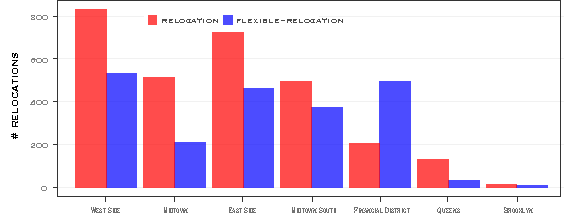
\includegraphics{figures/relocation_endzones.pdf}
	\caption{Contrast between preferred relocation destinations for drivers with 
	{\relocation} and {\relocationflexible} strategies on a representative day.}
	\label{fig:relocation_endzones}
\end{figure*}

\begin{figure}[h]
	\centering
	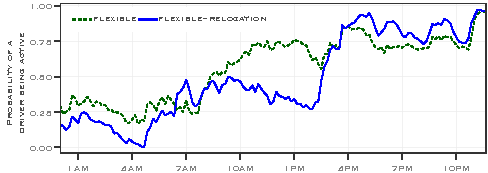
\includegraphics{figures/simulated_schedules.pdf}
	\caption{Active drivers with {\flexible} and {\relocationflexible}
	strategies at different times of a representative day.}
	\label{fig:simulated_schedules}
\end{figure}

Using the above input, we now evaluate our methodology. All our experiments were performed using a single process implementation of our algorithms on a 24-core 2.9GHz Intel Xeon E5 processor with 512GB memory. Computational time for the {\naive} and the {\relocation} strategies is less than a minute, and about 5 minutes for the {\flexible} and the {\relocationflexible} strategies. Uncertainty analysis (Section \ref{sec:effect_of_uncertainty}), with an off-the-shelf minimizer, takes around 3 hours.

\spara{Comparison of strategies}: First, we address the question: \textit{what is the best driver strategy?} Intuitively, it is clear that {\relocationflexible} is the best strategy, as it takes advantage of spatial as well as temporal variations in the passenger demand across NYC. In order to verify this intuition, we compare driver earnings across different strategies. Drivers following the {\naive} and the {\relocation} strategies are assumed to drive from 9 AM to 5 PM, a standard 8 hour workday, while those following the {\flexible} or the {\relocationflexible} strategies drive for a total of 8 hours each day with a flexible schedule.

Figure \ref{fig:daily_earnings} shows the average earnings achieved by 
the solution to {\originalproblem} by each of the strategies on different days of a representative week. We observe that all ``smart'' strategies consistently outperform {\naive};
as expected, {\relocationflexible} is consistently the strategy with the highest earnings.
Note that the {\relocationflexible} can lead to up to 100\% increase in the drivers'
earnings when compared to {\naive}.  
Thus, our strategies do exploit the spatial and the temporal variation in demand across NYC. The results also show
that for a part-time Uber driver, it is beneficial to drive midweek from Wednesday to Friday, than during weekends.

%Having established that the {\relocation}, {\flexible} and {\relocationflexible} strategies result in higher driver earnings than the {\naive} strategy, in the subsequent sections, we further analyze various aspects related to them.




\spara{Spatial dynamics of strategies}: 
Next, we address the question - \textit{what are the benefits of the {\relocate} action?} Figure \ref{fig:successful_heatmap} already shows the spatial variation in the demand across different NYC zones at different times of the day. Intuitively, this spatial variation can cause a disparity in the driver earnings based upon the zone of the driver. For example, drivers based in Manhattan should be expected 
to earn more than those based in Brooklyn due to persistently higher demand in Manhattan. Similarly, at different times of the day, drivers located within different parts of Manhattan itself will earn different amounts on account of temporal trends.


The {\relocation} strategy attempts to mitigate the location-based disparity in earnings by suggesting optimal relocation actions to drivers at various times of the day. Figure \ref{fig:earnings_heatmap} shows variation in earnings from 8 hour driving shifts starting morning 8 AM, noon 12 PM, evening 5 PM and night 10 PM, for drivers with different home zones. Not only do we observe that the {\relocation} strategy has a higher median than the {\naive}, but also, the inter-quartile range (IQR) is significantly narrower.\footnote{The lower and upper edges of the boxes in Figure \ref{fig:earnings_heatmap} indicate quartiles Q1 and Q3 respectively, and length of whisker is 1.5 times IQR.} This indicates that the location-based disparity in earnings for the {\naive} strategy is much larger than the {\relocation} strategy. Thus, we conclude that smart relocations throughout the day prevent a driver from becoming ``trapped'' in low-earning neighborhoods, translating 
into significant increases in the earnings. 
This may be counterintuitive to some drivers, as a {\relocate} action (essentially an empty ride) 
incurs cost to the driver. Yet, the results demonstrate that these actions, when timed appropriately, 
lead to earnings far higher than the costs they incur.

\spara{Temporal dynamics of strategies}: Intuitively, due to the periodicity of demand, we expect driver earnings to strongly depend on the time of the day they are driving. 
%We have also established via Figure \ref{fig:daily_earnings} that both of the flexible schedule strategies outperform their fixed schedule counterparts. 
Thus, we address the question: \textit{what is the best time of the day to drive in order to maximize earnings?} To answer this, we simulate 1000 drivers, each randomly assigned a home zone, for each of the {\flexible} and {\relocationflexible} strategies. 
We solve the {\originalproblem} problem for both strategies and create a recommended plan of action for the simulated drivers. 
Then, at every step of the simulation, a driver undertakes the personalized action recommended by the strategy, corresponding to
  the location, the time of the day and the budget remaining.


In Figure \ref{fig:simulated_schedules}, we plot the percentage of simulated drivers driving in the city at different times of the day. We observe a noticeable difference between the ``preferred'' driving schedules 
output by {\flexible} and {\relocationflexible}.
In particular, a high percentage of {\flexible} schedule drivers are active during the standard working hours of the day from 9AM to 6PM. In contrast, the number of active
drivers that follow {\relocationflexible} exhibits two distinct peaks, corresponding to the morning and the evening rush hours. Furthermore, over 50\% of {\relocationflexible} drivers use their driving budget in the later half of the day starting approximately at 3PM, continuing through till midnight. 
Since {\flexible} and {\relocationflexible} only differ in 
the {\relocate} action, all observed differences are due to this action.
Hence, we can  conclude that the {\relocate} action is most effective in the evening hours, thereby prompting higher active percentages of {\relocationflexible} drivers at that time.

\spara{Preferred relocation zones}: By simulating drivers, we can also compare the {\relocate} actions between drivers following {\relocation} strategy and those following {\relocationflexible} strategy. The contrast between popular destinations 
of {\relocate} actions for drivers following the two strategies can readily be seen in Figure \ref{fig:relocation_endzones}. 
We observe a contrast between the preferred relocation zones for drivers of these two strategies. 
Drivers following the {\relocation} strategy predominantly relocate themselves to the center of Manhattan. In contrast, the drivers following the {\relocationflexible} strategy do not exhibit a clear most-preferred relocation destination. Furthermore, the 
{\em number} of relocations performed by the {\relocation} strategy drivers, 
is, surprisingly, significantly higher than those performed by the {\relocationflexible} strategy drivers. 
This turns out to be due to the freedom of the work schedule of the latter, which allows them to drive 
  continuously during the hours of highest demand, reducing the frequency of {\relocate} actions they take. 

\subsection{Surge chasing}
\begin{figure}
	\centering
	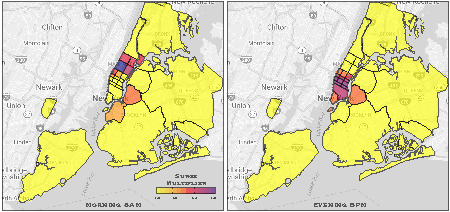
\includegraphics{figures/surge_heatmap.pdf}
	\caption{Active surge multiplier across NYC zones at different times of a representative day.}
	\label{fig:surge_heatmap}
\end{figure}

We now turn our attention to surge pricing. Surge pricing was a controversial feature of the Uber platform\footnote{Uber stopped displaying the `surge multiplier' prominently in its customer app since June 2016, instead now it displays price estimates after accounting for the surge~\cite{surge}.} 
aimed at matching supply with passenger demand by increasing prices at times of high demand. 
According to Uber, it incentivizes drivers to start driving during the peak hours in order to efficiently meet demand with 
  supply, albeit at a higher cost to passengers.
It also decreases demand, as the most price-sensitive customers drop out. 
%In fact, Uber prominently displays surge information to drivers on their Partner App.
%  in the form of a heat-map of surge multipliers in different geographical neighborhoods.

Figure \ref{fig:surge_heatmap} shows the active surge multiplier across different neighborhoods of NYC at 
different times of the day. 
This information is readily available to the drivers; however, due to uncertainty in the duration of surges 
  as well as the proprietary nature of Uber's surge pricing algorithm, 
  it is unclear whether drivers should relocate themselves to surging areas in order to maximize their earnings. 

Coupling our data on surge multipliers with other data, we are in a position to answer the question-- \textit{Should drivers engage in surge chasing?}
In order to do so, we evaluate earnings of simulated drivers in three scenarios viz., 
``no surge'' - where we disable the surge multiplier to compute earnings; ``surge'' - 
where the multiplier is used while calculating earnings; and ``surge chasing'' -
wherein a driver located in a non-surging zone always relocates to the zone with highest surge multiplier. 
Simulated driver earnings in these three scenarios for each of the strategies are shown in Figure {\ref{fig:simulated_earnings}}. 
We observe that blind ``surge chasing'' leads to lower earnings irrespective of the strategy being followed. 
Figure \ref{fig:simulated_earnings} reinforces our previous observation regarding the high variance of the {\naive} strategy. 
At times, drivers following the {\naive} strategy with surge multiplier enabled may earn less than when it is disabled. 
For other strategies, ``surge chasing'' consistently fails to provide any tangible benefits as compared to 
following the pre-determined strategy. We conclude that actively and blindly chasing the surge is an ill-advised 
strategy and may lead to losses. Furthermore, surges last for short durations and an unsuccessful surge chase 
may land a driver in a sub-optimal location with respect to longer term earnings. 

\subsection{Effect of uncertainty}
\label{sec:effect_of_uncertainty} 
Our experiments indicate that our strategies always outperform a {\naive} strategy that is likely prevalent 
among Uber drivers. However, all our strategies use historical data. Consequently, 
our results can potentially be sensitive to perturbations of the empirically-observed transition matrices. 
Thus, we can only conclude that our results are robust if
the drivers following one of the {\relocation}, {\flexible} and {\relocationflexible} strategies
have higher earnings than those following {\naive} even when the input data is perturbed.
\begin{figure}
	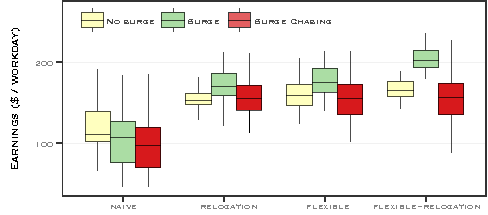
\includegraphics{figures/simulated_earnings.pdf}
	\caption{Exploring surge: Simulated earnings for drivers across different strategies on a representative day.}
	\label{fig:simulated_earnings}
\end{figure}

Hence, the question we have to address is the following: 
\textit{Are the conclusions we drew above robust to perturbations of the empirical transition matrices?} We do so using
the framework we developed in Section \ref{sec:sensitivity}:  
we solve the {\robustproblem} problem for each of the four strategies for increasing levels of uncertainty ($\alpha$).

Figure \ref{fig:uncertainty_evolution} shows the effect of increasing uncertainty on the earnings of drivers for
    each of the four strategies.  We observe two main takeaways.  First, we find that all strategies
   suffer a loss under small amounts of uncertainty, even at levels of $\alpha$ in the range of 0.02, so all
   strategies are tuned closely to the empirical data.  
However, all strategies then remain resilient to a wide range of additional uncertainty, and we find that
   the {\relocation}, {\flexible} and {\relocationflexible} strategies are most tolerant to uncertainty 
  in the input transition matrices. 
Interestingly, even with 99\% uncertainty, the {\relocationflexible} strategy significantly outperforms 
  the {\naive} strategy with no uncertainty.
This observation further supports our claim that being strategic using historical data can significantly improve driver 
  earnings in on-demand ridesharing platforms. 

\begin{figure}[hb]
	\centering
	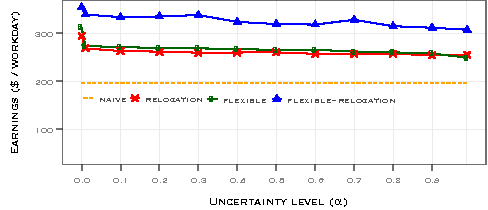
\includegraphics{figures/uncertainty_evolution.pdf}
	\caption{Sensitivity to uncertainty in parameters.}
	\label{fig:uncertainty_evolution}
\end{figure}

% \subsection{\textsc{RewardsMatrix}}

% The data gathered in the previous section gives us a matrix of driver earnings, \matr{E}, from passengers while traveling between any two zones in the city. We also get a costs matrix, \matr{C}, whose each entry, $c(i,j) \leq 0$, denotes the sundry expenses of traveling from zone $i$ to zone $j$, dependent on distance and traffic at the given time. The travel costs can result in negative net rewards in the {\gohome} and {\relocate} actions, violating the assumption from Section \ref{sec:problem_setup} that $r(i,j) \geq 0$. In this section, we describe the construction of \textsc{RewardsMatrix}, {\rewardsmatrix}, corresponding to each driver action compliant with our assumptions.

% \subsubsection{\textsc{Modifying the CostsMatrix}}
% If $min\_cost$ is the minimum entry in the matrix \matr{C}, each entry of the modified costs matrix, \matr{C'} is calculated as,
% \begin{equation}
% c'(i,j) = c(i,j) - min\_cost
% \end{equation}
% As a result of the above modification, $\forall i,j : c'(i,j) \geq 0$.

% \subsubsection{\textsc{RewardsMatrix}}
% In order to be compliant with the assumption in Section \ref{sec:problem_setup}, we define two kinds of \textsc{RewardsMatrix}, one for the action {\getpassenger} and another for the actions {\gohome} and {\relocate}.

% \begin{itemize}
% 	\item For the {\getpassenger} action, we define the rewards matrix as,
% 	\begin{equation}
% 		r(i,j) = e(i,j) + c'(i,j) 
% 	\end{equation}
% 	\item For the {\gohome} and {\relocate} actions, the rewards matrix is same as the modified costs matrix.
% 	\begin{equation}
% 		r(i,j) = c'(i,j)
% 	\end{equation}
% \end{itemize}
% In both cases, we set the diagonal entries of the matrix to zero i.e., $\forall i: r(i,i) = 0$.

% It should be noted that this modification does not affect the optimal action choice in any strategy. It merely ensures that the input vectors to the Bisection Algorithm from Section \ref{sec:sensitivity} are always non-negative vectors. Furthermore, while calculating the actual {\totalexpectedearnings} of a driver, we can backtrack these modifications.

% \subsection{\textsc{Comparing robust and nominal strategies}}
% In this section, we compare various strategies. When we choose, $\beta = \betamax$, there is no uncertainty, and we get solution computed via the classical Bellman recursion; referred to as nominal strategy. The robust strategy corresponds to solving the MDP with varying values of $\beta$.

% \subsection{\textsc{Effect of Inaccuracy is uncertainty level}}
% The previous section assumes that, in the robust case, we are able to estimate exactly the precise value of the uncertainty level. In practice, the parameter $\beta$ also has to be estimated. In this section, we study the sensitivity of the robust approach with respect to inaccuracies in the uncertainty parameter $\beta$.

%!TEX root = uber.tex

\begin{frame}{Conclusion}
\begin{itemize}
	\item Ride-hailing platform's matching algorithms may not be optimal for drivers.
	\item We propose a deployable methodology for maximizing driver earnings.
	\pause
	\vspace{1cm}
	\item \alert{Need for co-ordination when a significant percentage of driver population becomes strategic.}
\end{itemize}
\end{frame}
%!TEX root = main.tex

\mpara{Acknowledgments:} This work was supported by NSF awards: CAREER 1253393
and III 1421759. The authors also thank the anonymous reviewers for their helpful comments.
\bibliographystyle{ACM-Reference-Format}
\balance
\bibliography{sigproc} 

\end{document}
